\documentclass{article}
\usepackage[T1]{fontenc}

\usepackage{amssymb}
\usepackage{courier}
\usepackage{fancyhdr}
\usepackage{fancyvrb}
\usepackage[top=.75in, bottom=.75in, left=.75in,right=.75in]{geometry}
\usepackage{graphicx}
\usepackage{lastpage}
\usepackage{listings}
\lstset{basicstyle=\small\ttfamily}
\usepackage{mdframed}
\usepackage{parskip}
\usepackage{soul}
\usepackage{tabularx}
\usepackage{textcomp}
\usepackage{upquote}
\usepackage{xcolor}

% http://www.monperrus.net/martin/copy-pastable-ascii-characters-with-pdftex-pdflatex
\lstset{
upquote=true,
columns=fullflexible,
keepspaces=true,
literate={*}{{\char42}}1
         {-}{{\char45}}1
         {^}{{\char94}}1
}
\lstset{
  moredelim=**[is][\color{blue}\bf\small\ttfamily]{@}{@},
}

% http://tex.stackexchange.com/questions/40863/parskip-inserts-extra-space-after-floats-and-listings
\lstset{aboveskip=6pt plus 2pt minus 2pt, belowskip=-4pt plus 2pt minus 2pt}


% Python syntax in listings
\definecolor{pgreen}{rgb}{0,0.5,0}
\lstdefinestyle{Python}{
  language=Python,  
  aboveskip=3mm,
  belowskip=3mm,
  numbers=left,
  numbersep=8pt,
  numberstyle=\small\ttfamily\color{gray},
  basicstyle={\small\ttfamily},
  commentstyle=\color{gray},
  showstringspaces=false,
  tabsize=4,
    showspaces=false,
    showtabs=false,
    breaklines=true,
    showstringspaces=false,
    breakatwhitespace=true,
    commentstyle=\color{pgreen},
    keywordstyle=\color[HTML]{A71D5D},
    stringstyle=\color[HTML]{0086B3},
    basicstyle=\ttfamily
}


\usepackage[colorlinks,urlcolor={blue}]{hyperref}
\usepackage[capitalise,nameinlink,noabbrev]{cleveref}
\crefname{section}{Question}{Questions}
\Crefname{section}{Question}{Questions}

\begin{document}


\fancyfoot[L]{\color{gray} C4CS -- W'18}
\fancyfoot[R]{\color{gray} Revision 1.0}
\fancyfoot[C]{\color{gray} \thepage~/~\pageref*{LastPage}}
\pagestyle{fancyplain}

\title{\textbf{Homework 7\\Unit Testing and Python}}
\author{\textbf{\color{red}{Due: Wednesday, March 7th, 11:59PM (Hard Deadline)}}}
\date{}
\maketitle


\section*{Submission Instructions}
When you are done, submit a link to your GitHub repository here: \url{https://goo.gl/forms/56zbjqh1YnnregSF3}


\bigskip

\begin{mdframed}\centering
For this assignment, we will build on the RPN calculator from lecture.
\end{mdframed}



\section{Continuous Integration}
One of the neat elements of modern software development is \emph{continuous
  integration}. CI technologies automatically run test suites throughout the
development process and help prevent bugs from creeping in.

\subsection{The Setup}

While GitLab does support CI, it's not quite set up and working here at
Michigan yet, so we'll do this next bit using
\href{https://github.com}{GitHub} instead.
We'll use \href{https://travis-ci.org/}{Travis CI} as our CI platform.

\begin{enumerate}
  \item As a first step, create accounts on both of these platforms -- do
    GitHub first, Travis CI will use your GitHub account.
  \item Next, create a new repository named \textbf{c4cs-w18-rpn} on GitHub.
  \item Like submitting for attendance, we'll follow the directions from
    GitHub for ``\dots{}or push an existing repository from the command
    line''. \emph{However}, we already have a remote named ``origin'', so
    we'll need to change the commands just a little:
    \begin{itemize}
      \item \texttt{git remote add \textbf{github} https://github.com/\textbf{your-github-username}/c4cs-w18-rpn.git}
      \item \texttt{git push -u \textbf{github} master}
    \end{itemize}
  \item Refresh the GitHub page in your browser -- you should see your code!
  \item Now that we have a repository, we need to enable Travis CI for this
    repository. Visit \url{https://travis-ci.org/profile} and enable Travis
    for the repository you just made.
    \begin{itemize}
      \item You may need to click the ``Sync Account'' button in the top
        right if it doesn't immediately show up
    \end{itemize}
\end{enumerate}

\emph{Note: Final versions of \texttt{rpn.py} and \texttt{test\_rpn.py} from
  lecture are on the course homepage (\url{https://c4cs.github.io/}).}

\newpage

\subsection{The Part You Have to Figure Out}

Travis uses a file named \texttt{.travis.yml}\footnote{%
  Note the leading period for this file. Remember that makes it a \emph{hidden
    file}. This means it won't show up if you just run \texttt{ls}. You have
  to run \texttt{ls -a} (think ``all'') to see it. Other than this little
  quirk, hidden files are like any other. You can edit them with any text
  editor, no fanciness.
} to figure out what it needs to do. You will need to create this file, commit
it, and then run \texttt{git push} to push that commit to GitHub. Once you
push, Travis will automatically start running.

It is very likely that Travis will error on your first try. That's fine. Just
make some changes to \texttt{.travis.yml}, commit, and push again.

The things you'll have to tell Travis in your configuration file:
\begin{enumerate}
  \item This is a Python project
  \item This project requires Python3 (any version of Python3, but 3.5 is a
    good choice)
  \item How to run your tests
\end{enumerate}

A few links that may help:
\begin{itemize}
  \item Wikipedia on YAML for a syntax primer: \url{https://en.wikipedia.org/wiki/YAML}
  \item Travis CI's getting started guide:
    \url{https://docs.travis-ci.com/user/getting-started/#To-get-started-with-Travis-CI\%3A}
  \item Travis CI's guide for Python:
    \url{https://docs.travis-ci.com/user/languages/python/}
  \item Travis Lint: \url{http://lint.travis-ci.org/}
    \begin{itemize}
      \item A \emph{linter} is a tool that checks code for syntax and style
        problems. It validates that things are correct, make sense, and gives
        feedback on how to make your code better.
      \item I'm really bad at writing YAML, the syntax has just never made
        sense to me, so I find this really useful
    \end{itemize}
\end{itemize}

When you've got everything working,
\texttt{https://travis-ci.org/\textbf{your-github-username}/c4cs-w18-rpn}
should look something like this:

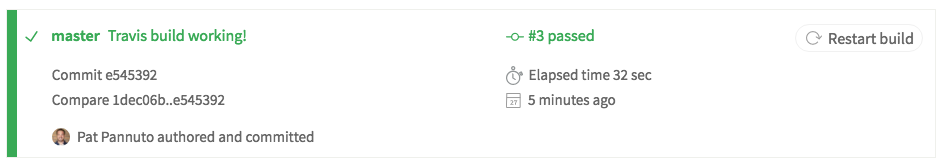
\includegraphics[width=\linewidth]{travis-rpn-working}


\vfill

\begin{mdframed}\centering
For this class, we're happy to do everything publicly. If you use GitHub and
Travis CI for other class projects
\textbf{\emph{\large You MUST create PRIVATE repositories}}.

You can do this for free as a student, grab a copy of the
\href{https://education.github.com/pack}{GitHub Student Developer Pack} to get
started.

{\color{red}
  For most EECS classes at Michigan, posting your code online (e.g. a public
  repository) is an honor code violation. You may be subject to failing the
  project, failing the course, or other penalties.

  \textbf{\emph{\Large DO NOT PUT CODE FOR OTHER EECS CLASSES IN PUBLIC REPOSITORIES}}
}
\end{mdframed}










\newpage

\section{Let's do some test-driven-development}

\subsection{Make the test}
Add a test to your test suite for the exponentiation operator (the carat:
\texttt{\^{}}). Once you have finished your test, commit and push your test.
Verify that your Travis build \textbf{fails} (you have not implemented carat
support yet!). Fix your Travis setup if you need to.

\subsection{Add the implementation}
Add support to your RPN calculator for exponentiation. Commit, push,
and verify that your CI build is ``green'' (the tests pass).


\section*{Submission Instructions}
When you are done, submit a link to your GitHub repository to the link given at
the beginning of the homework.

\end{document}








%%%%%%%%%%%%%%%%%%%%%%%%%%%%%%%%%%%%%%%%%%%%%%%%%%%%%%%%%%%%%%%%%%%%%%%%%%
\begin{comment}

\section{Leveraging Classes}

Classes, objects, polymorphism, inheritance, and all the rest of that
vocabulary can seem a little intimidating sometimes, especially when you are
first starting.

\emph{Note for the 280 folks: This is coming slightly before object-oriented
  materials in 280.  You \textbf{do not} need to deeply understand objects,
  Python classes, etc to do this assignment. The goal is to show a simple
  example and hopefully give some intuition for when you do cover objects in
  280.}

Let's take a look at how we can convert the template from lecture (left) to make a
Calculator object (right):

\begin{minipage}{.49\textwidth}
\begin{lstlisting}[style=Python]
#!/usr/bin/env python3

def calculate(string):
    pass
def main():

    while True:
        calculate(input("rpn> "))
if __name__ == '__main__':
    main()
\end{lstlisting}
\end{minipage}
\begin{minipage}{.49\textwidth}
\begin{lstlisting}[style=Python]
#!/usr/bin/env python3
class Calculator:
    def calculate(self, string):
        pass
def main():
    calc = Calculator()
    while True:
        calc.calculate(input("rpn> "))
if __name__ == '__main__':
    main()
\end{lstlisting}
\end{minipage}

The changes are
\begin{enumerate}
  \item Add the line \texttt{class Calculator:}, which is defining a new type
    of object, a Calculator
  \item Indent the \texttt{calculate} function and its whole function body to
    make that function part of the new Calculator object, instead of being a
    global function
  \item Change the \texttt{calculate} function to take a \texttt{self}
    argument
    \begin{itemize}
      \item \texttt{self} is a reference to the current calculator instance,
        it's more or less the \texttt{this} pointer from \texttt{C++}
      \item If none of that made sense, don't worry, you can just ignore
        \texttt{self} for now
    \end{itemize}
  \item Create an \emph{instance} of a Calculator object on line 6
  \item On line 8, \texttt{calculate} is no longer a global function, so we
    have to ask the \texttt{calc} object we got on line 6 to call
    \texttt{calculate}
\end{enumerate}

\end{comment}
